\documentclass[aspectratio=169, 10pt]{beamer}

\usepackage{bm} % bold math
\usepackage{fontspec}
\usepackage{minted}
\usepackage{pgf-pie}
\usepackage{tikz}

% Custom commands and environments
\makeatletter
\newcommand\version[1]{\renewcommand\@version{#1}}
\newcommand\@version{}
\def\insertversion{\@version}

\newcommand\course[1]{\renewcommand\@course{#1}}
\newcommand\@course{}
\def\insertcourse{\@course}

\newcommand\coursetitle[1]{\renewcommand\@coursetitle{#1}}
\newcommand\@coursetitle{}
\def\insertcoursetitle{\@coursetitle}

\newcommand\lecturenumber[1]{\renewcommand\@lecturenumber{#1}}
\newcommand\@lecturenumber{}
\def\insertlecturenumber{\@lecturenumber}
\makeatother

\newcommand{\slidetitle}[1]{{\xbseries \large \structure{#1}} \bigskip}
\newcommand{\term}[1]{{\color{blue} #1}}
\newcommand{\leftspace}{\hspace{1em}}
\newcommand{\inlinearrow}{
  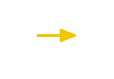
\begin{tikzpicture}[baseline]
    \node [anchor=base] (x) {};
    \draw [rawarrow] (x.mid west) -- ($(x.mid west) + (2em,0)$);
  \end{tikzpicture}
}

\newenvironment{slide}
{\begin{frame}[fragile,environment=slide]\vskip0pt plus 1filll}
{\vskip0pt plus 1filll\end{frame}}

% LaTeX

\setlength{\leftmargini}{1em}

% Common Information

\author{Jon Eyolfson}
\course{ECE 353}
\coursetitle{Systems Software}
\date{2024 Winter}

% fontspec

\defaultfontfeatures{Ligatures=TeX}
% \setmainfont{Domine}
\setsansfont{Inter}[
  FontFace={ul}{n}{Font=*-Thin},
  FontFace={el}{n}{Font=*-ExtraLight},
  FontFace={l}{n}{Font=*-Light},
  FontFace={sb}{n}{Font=*-SemiBold},
  FontFace={eb}{n}{Font=*-ExtraBold},
  FontFace={xb}{n}{Font=*-Black},
]
\setmonofont[Contextuals=AlternateOff, Ligatures=TeXOff]{Iosevka}[
  FontFace={xb}{n}{Font=*-Heavy},
]

%% Font Weights

\DeclareRobustCommand{\ulseries}{\fontseries{ul}\selectfont}
\DeclareTextFontCommand{\textul}{\ulseries}
\DeclareRobustCommand{\elseries}{\fontseries{el}\selectfont}
\DeclareTextFontCommand{\textel}{\elseries}
\DeclareRobustCommand{\lseries}{\fontseries{l}\selectfont}
\DeclareTextFontCommand{\textl}{\lseries}
\DeclareRobustCommand{\sbseries}{\fontseries{sb}\selectfont}
\DeclareTextFontCommand{\textsb}{\sbseries}
\DeclareRobustCommand{\ebseries}{\fontseries{eb}\selectfont}
\DeclareTextFontCommand{\texteb}{\ebseries}
\DeclareRobustCommand{\xbseries}{\fontseries{xb}\selectfont}
\DeclareTextFontCommand{\textxb}{\xbseries}

% tikz

\usetikzlibrary{
  arrows,
  arrows.meta,
  automata,
  backgrounds,
  calc,
  decorations.pathreplacing,
  matrix,
  positioning,
  overlay-beamer-styles,
  shapes,
  shapes.multipart,
  tikzmark,
}

\tikzstyle{rawarrow} = [
  -{Latex[round]},
  line width=1pt,
  yellow,
  shorten >=3pt,
  shorten <=3pt,
  font=\small,
  text=black,
]

\tikzstyle{arrow} = [
  -{Latex[round]},
  line width=1pt,
  yellow,
  shorten >=3pt,
  shorten <=3pt,
  transform canvas={yshift=3pt},
  font=\small,
  text=black,
]

\newcommand{\tikzmarkcoord}[1]{([yshift=3pt]pic cs:#1)}

% minted

\setminted{style=eyolfson, fontsize=\small, escapeinside=||}
\setmintedinline{fontsize=\normalsize}

% hyperref

\hypersetup{colorlinks, urlcolor=blue}

% beamer
\setbeamersize{text margin left=16mm, text margin right=16mm}
\setbeamertemplate{itemize items}[circle]
\setbeamercolor{item}{fg=black}
\setbeamercolor{structure}{fg=darkblue}
\setbeamerfont{frametitle}{series=\bfseries, parent=structure}
\setbeamertemplate{navigation symbols}{}
\setbeamertemplate{headline}{}
\setbeamertemplate{footline}{
  \begin{tikzpicture}[
    remember picture,
    overlay,
    shift={(current page.south west)},
  ]
    \path [fill=gray] (144mm, 0) -- (160mm, 16mm) -- (160mm, 0);
    \node [inner sep=3.5mm, outer sep=0, text=black, anchor=base east,
           align=right, yshift=3.5mm]
          at (current page.south east) {\ttfamily \small \insertframenumber{}};
  \end{tikzpicture}
}
\setbeamertemplate{title page}{
  \begin{tikzpicture}[
    remember picture,
    overlay,
    shift={(current page.south west)},
    background rectangle/.style={fill=darkblue},
    show background rectangle,
  ]
    \node [anchor=center, align=center, text=white, text width=40mm, scale=3.2]
          at (\paperwidth / 2, \paperheight * 2 / 3)
          {\xbseries \inserttitle{}};
    \node [anchor=base west, align=left, inner sep=0, text=white, yshift=2.5mm]
          at (16mm, \paperheight / 3)
          {\insertdate{} \insertcourse{}: \insertcoursetitle{}};
    \node [anchor=base west, align=left, inner sep=0, text=white, yshift=-2.5mm]
          at (16mm, \paperheight / 3)
          {\insertauthor};
    \node [anchor=base east, align=right, inner sep=0, text=white, yshift=2.5mm]
          at (144mm, \paperheight / 3)
          {Lecture \insertlecturenumber{}};
    \node [anchor=base east, align=right, inner sep=0, text=white,
           yshift=-2.5mm]
          at (144mm, \paperheight / 3)
          {\ttfamily \insertversion{}};
    \node [align=center, anchor=south, inner sep=0, text=white, yshift=3.5mm]
          (license) at (\paperwidth / 2, 0)
          {\fontsize{7pt}{7pt}\selectfont This  work is licensed under a
           \href{http://creativecommons.org/licenses/by-sa/4.0/}
                {\color{lightblue} Creative Commons Attribution-ShareAlike 4.0
                 International License}};
  \end{tikzpicture}
}

% xcolor

%% Primary Colour

\definecolor{pantone655}{RGB}{0, 42, 92} % #002a5c
\colorlet{darkblue}{pantone655}

%% Secondary Colours

\definecolor{pantone633}{RGB}{0, 139, 176} % #008bb0
\colorlet{blue}{pantone633}

\definecolor{pantonewarmred}{RGB}{220, 70, 51} % #dc4633
\colorlet{red}{pantonewarmred}

\definecolor{pantone3285}{RGB}{0, 161, 137} % #00a189
\colorlet{cyan}{pantone3285}

\definecolor{pantone7722}{RGB}{13, 83, 77} % #0d534d
\colorlet{darkcyan}{pantone7722}

\definecolor{pantone376}{RGB}{141, 191, 46} % #8dbf2e
\colorlet{green}{pantone376}

\definecolor{pantone2613}{RGB}{109, 36, 122} % #6d247a
\colorlet{violet}{pantone2613}

\definecolor{pantone2985}{RGB}{111, 199, 234} % #6fc7ea
\colorlet{lightblue}{pantone2985}

\definecolor{pantone227}{RGB}{171, 19, 104} % #ab1368
\colorlet{magenta}{pantone227}

\definecolor{pantone7406}{RGB}{241, 197, 0} % #f1c500
\colorlet{yellow}{pantone7406}

%% Neutrals

\definecolor{pantonecoolgray2}{RGB}{208, 209, 201} % #d0d1c9
\colorlet{gray}{pantonecoolgray2}


\lecturenumber{13}
\title{Page Table\\Implementation}
\version{2.0.0}

\begin{document}
  \begin{frame}[plain, noframenumbering]
    \titlepage
  \end{frame}

  \begin{slide}

    \slidetitle{Processes Use A Register Like \texttt{satp} to Set the Root Page Table}

    \centering
    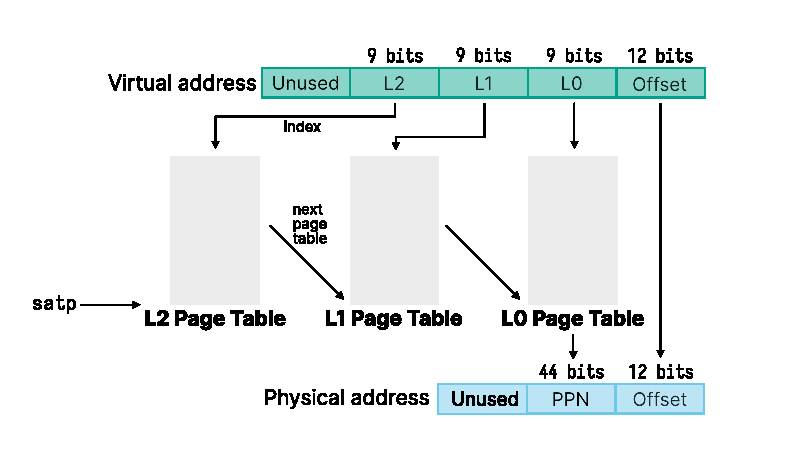
\includegraphics{../12-page-tables/multi-level-page-table.eps}

  \end{slide}

  \begin{slide}
    
    \slidetitle{Alignment: Memory Eventually Lines Up with Byte 0}

    If pages are \textit{4096 byte aligned} in memory is means pages always
    start when the lower 12 bits are zero, in computing we like alignment
    \medskip

    If a page started at address \texttt{0x7C00} its last byte would be at
    address \texttt{0x8BFF}
    \medskip

    Instead, a page would start at \texttt{0x7000} and end at \texttt{0x7FFF}
    \bigskip

    Question: Is address \texttt{0xEC} 8 byte aligned?
  \end{slide}

  \begin{slide}
    
    \slidetitle{Let's Simulate an MMU}

    \texttt{lectures/12-page-tables} in the \texttt{materials} repository
    \medskip

    Remember each process would have its own unique root page table

  \end{slide}

  \begin{slide}
    
    \slidetitle{How Many Page Tables Do We Need?}

    Let's assume our program uses 512 pages
    \medskip

    What's the minimum number of page tables we need?
    \medskip

    What's the maximum number of page tables?

  \end{slide}

  \begin{slide}

    \slidetitle{How Many Levels Do I Need?}

    Assume we have a 32-bit virtual address with a page size of 4096 bytes

    \leftspace{}and a PTE size of 4 bytes
    \medskip

    We want each page table to fit into a single page

    \leftspace{}Find the number of PTEs we could have in a page ($\mathsf{2^{10}}$)

    \leftspace{}\leftspace{}$\mathsf{log_2(\# PTEs\ per\ Page)}$ is the number of bits to index a page table
    \medskip

    $\mathsf{\# Levels = \lceil \frac{Virtual\ Bits - Offset\ Bits}{Index\ Bits} \rceil}$
    \medskip

    \onslide<2->{$\mathsf{\# Levels = \lceil \frac{32 - 12}{10} \rceil = 2}$}

  \end{slide}

  \begin{slide}

    \slidetitle{Using the Page Tables for Every Memory Access is Slow}

    We need to follow pointers across multiple levels of page tables!
    \medskip

    We'll likely access the same page multiple times
    
    (close to the first access time)
    \medskip

    A process may only need a few VPN $\rightarrow$ PPN mappings at a time
    \medskip

    Our solution is another computer science classic: caching

  \end{slide}

  \begin{slide}

    \slidetitle{A Translation Look-Aside Buffer (TLB) Caches PTEs}

    \centering
    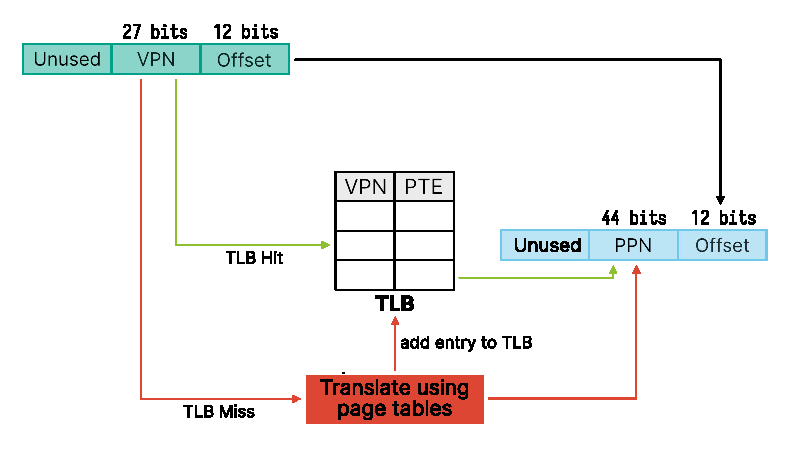
\includegraphics{tlb.eps}

  \end{slide}

  \begin{slide}

    \slidetitle{Effective Access Time (EAT)}

    Assume a single page table
    
    \leftspace{}(there's only one additional memory access in the page table)
    \medskip

    $\mathsf{TLB\_Hit\_Time = TLB\_Search + Mem}$

    $\mathsf{TLB\_Miss\_Time = TLB\_Search + 2 \times Mem}$

    $\mathsf{EAT = \alpha \times TLB\_Hit\_Time + (1 - \alpha) \times TLB\_Miss\_Time}$
    \medskip

    If $\mathsf{\alpha = 0.8}$, $\mathsf{TLB\_Search = 10\ ns}$, and accesses take 100 ns, calculate EAT

    \leftspace{}$\mathsf{EAT = 0.8 \times 110\ ns + 0.2 \times 210\ ns}$

    \leftspace{}$\mathsf{EAT = 130\ ns}$

  \end{slide}

  \begin{slide}

    \slidetitle{Context Switches Require Handling the TLB}

    You can either flush the cache, or attach a process ID to the TLB
    \medskip

    Most implementation just flush the TLB

    \leftspace{}RISC-V uses a \texttt{sfence.vma} instruction to flush the TLB
    \medskip

    On x86 loading the base page table will also flush the TLB

  \end{slide}

  \begin{slide}

    \slidetitle{TLB Testing}

    Check out \texttt{lectures/13-page-table-implementation/test-tlb}

    \leftspace{}(you may need to \texttt{git submodule update --init --recursive})
    \medskip

    \texttt{./test-tlb <size> <stride>}

    \leftspace{}Creates a <size> memory allocation and acccesses it every <stride> bytes
    \medskip

    Results from my laptop:
    \begin{minted}{console}
> ./test-tlb 4096 4        
  1.93ns (~7.5 cycles)
> ./test-tlb 536870912 4096
155.51ns (~606.5 cycles)
> ./test-tlb 16777216 128  
 14.78ns (~57.6 cycles)
    \end{minted}

  \end{slide}

  \begin{slide}

    \slidetitle{Use \texttt{sbrk} for Userspace Allocation}

    This call grows or shrinks your heap (the stack has a set limit)
    \medskip

    For growing, it'll grab pages from the free list to fulfill the request

    \leftspace{}The kernel sets \texttt{PTE\_V} (valid) and other permissions
    \medskip

    In memory allocators this is difficult to use, you'll rarely shrink the heap

    \leftspace{}It'll stay claimed by the process, and the kernel cannot free
    pages
    \medskip

    Memory allocators use \texttt{mmap} to bring in large blocks of virtual
    memory

  \end{slide}

  \begin{slide}

    \slidetitle{The Kernel Initializes the Processs' Address Space}

    \centering
    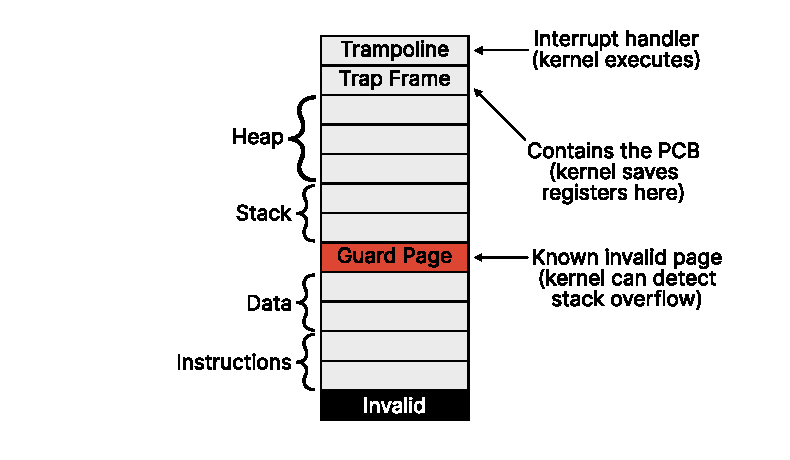
\includegraphics{address-space.eps}

  \end{slide}

  \begin{slide}

    \slidetitle{The Kernel Can Provide Fixed Virtual Addresses}

    It allows the process to access kernel data without using
    a system call
    \medskip

    For instance \texttt{clock\_gettime} does not do a system call

    \leftspace{}It just reads from a virtual address mapped by the kernel

  \end{slide}

  \begin{slide}

    \slidetitle{Page Faults Allow the Operating System to Handle Virtual Memory}

    Page faults are a type of exception for virtual memory access

    \leftspace{}Generated if it cannot find a translation, or permission check fails
    \medskip

    This allows the operating system to handle it

    \leftspace{}We could lazily allocate pages, implement copy-on-write, or swap to disk

  \end{slide}

  \begin{slide}

    \slidetitle{Page Tables Translate Virtual to Physical Addresses}

    The MMU is the hardware that uses page tables, which may:

    \begin{itemize}
      \item Be a single large table (wasteful, even for 32-bit machines)
      \item Use the kernel allocated pages from a free list
      \item Be a multi-level to save space for sparse allocations
      \item Use a TLB to speed up memory accesses
    \end{itemize}

  \end{slide}

\end{document}
